% Created 2025-10-13 ma 17:26
% Intended LaTeX compiler: pdflatex
\documentclass[12pt]{article}

%%%% settings when exporting code %%%% 

\usepackage{listings}
\lstdefinestyle{code-small}{
backgroundcolor=\color{white}, % background color for the code block
basicstyle=\ttfamily\small, % font used to display the code
commentstyle=\color[rgb]{0.5,0,0.5}, % color used to display comments in the code
keywordstyle=\color{black}, % color used to highlight certain words in the code
numberstyle=\ttfamily\tiny\color{gray}, % color used to display the line numbers
rulecolor=\color{black}, % color of the frame
stringstyle=\color[rgb]{0,.5,0},  % color used to display strings in the code
breakatwhitespace=false, % sets if automatic breaks should only happen at whitespace
breaklines=true, % sets automatic line breaking
columns=fullflexible,
frame=single, % adds a frame around the code (non,leftline,topline,bottomline,lines,single,shadowbox)
keepspaces=true, % % keeps spaces in text, useful for keeping indentation of code
literate={~}{$\sim$}{1}, % symbol properly display via latex
numbers=none, % where to put the line-numbers; possible values are (none, left, right)
numbersep=10pt, % how far the line-numbers are from the code
showspaces=false,
showstringspaces=false,
stepnumber=1, % the step between two line-numbers. If it's 1, each line will be numbered
tabsize=1,
xleftmargin=0cm,
emph={anova,apply,class,coef,colnames,colNames,colSums,dim,dcast,for,ggplot,head,if,ifelse,is.na,lapply,list.files,library,logLik,melt,plot,require,rowSums,sapply,setcolorder,setkey,str,summary,tapply},
aboveskip = \medskipamount, % define the space above displayed listings.
belowskip = \medskipamount, % define the space above displayed listings.
lineskip = 0pt} % specifies additional space between lines in listings
\lstset{style=code-small}
%%%% packages %%%%%

\usepackage[utf8]{inputenc}
\usepackage[T1]{fontenc}
\usepackage{lmodern}
\usepackage{textcomp}
\usepackage{color}
\usepackage{graphicx}
\usepackage{grffile}
\usepackage{wrapfig}
\usepackage{rotating}
\usepackage{longtable}
\usepackage{multirow}
\usepackage{multicol}
\usepackage{changes}
\usepackage{pdflscape}
\usepackage{geometry}
\usepackage[normalem]{ulem}
\usepackage{amssymb}
\usepackage{amsmath}
\usepackage{amsfonts}
\usepackage{dsfont}
\usepackage{array}
\usepackage{ifthen}
\usepackage{hyperref}
\usepackage{natbib}
\RequirePackage{setspace} % to modify the space between lines - incompatible with footnote in beamer
\renewcommand{\baselinestretch}{1.1}
\geometry{a4paper, left=10mm, right=10mm, top=10mm}
\usepackage{titlesec}
\usepackage{etoolbox}

\makeatletter
\patchcmd{\ttlh@hang}{\parindent\z@}{\parindent\z@\leavevmode}{}{}
\patchcmd{\ttlh@hang}{\noindent}{}{}{}
\makeatother
\RequirePackage{colortbl} % arrayrulecolor to mix colors
\definecolor{myorange}{rgb}{1,0.2,0}
\definecolor{mypurple}{rgb}{0.7,0,8}
\definecolor{mycyan}{rgb}{0,0.6,0.6}
\newcommand{\lightblue}{blue!50!white}
\newcommand{\darkblue}{blue!80!black}
\newcommand{\darkgreen}{green!50!black}
\newcommand{\darkred}{red!50!black}
\definecolor{gray}{gray}{0.5}
\hypersetup{
citecolor=[rgb]{0,0.5,0},
urlcolor=[rgb]{0,0,0.5},
linkcolor=[rgb]{0,0,0.5},
}
\newenvironment{note}{\small \color{gray}\fontfamily{lmtt}\selectfont}{\par}
\newenvironment{activity}{\color{orange}\fontfamily{qzc}\selectfont}{\par}
\RequirePackage{pifont}
\RequirePackage{relsize}
\newcommand{\Cross}{{\raisebox{-0.5ex}%
{\relsize{1.5}\ding{56}}}\hspace{1pt} }
\newcommand{\Valid}{{\raisebox{-0.5ex}%
{\relsize{1.5}\ding{52}}}\hspace{1pt} }
\newcommand{\CrossR}{ \textcolor{red}{\Cross} }
\newcommand{\ValidV}{ \textcolor{green}{\Valid} }
\usepackage{stackengine}
\usepackage{scalerel}
\newcommand\Warning[1][3ex]{%
\renewcommand\stacktype{L}%
\scaleto{\stackon[1.3pt]{\color{red}$\triangle$}{\tiny\bfseries !}}{#1}%
\xspace
}
\RequirePackage{fancyvrb}
\DefineVerbatimEnvironment{verbatim}{Verbatim}{fontsize=\small,formatcom = {\color[rgb]{0.5,0,0}}}
\definecolor{grayR}{HTML}{8A8990}
\definecolor{grayL}{HTML}{C4C7C9}
\definecolor{blueM}{HTML}{1F63B5}
\newcommand{\Rlogo}[1][0.07]{
\begin{tikzpicture}[scale=#1]
\shade [right color=grayR,left color=grayL,shading angle=60]
(-3.55,0.3) .. controls (-3.55,1.75)
and (-1.9,2.7) .. (0,2.7) .. controls (2.05,2.7)
and (3.5,1.6) .. (3.5,0.3) .. controls (3.5,-1.2)
and (1.55,-2) .. (0,-2) .. controls (-2.3,-2)
and (-3.55,-0.75) .. cycle;

\fill[white]
(-2.15,0.2) .. controls (-2.15,1.2)
and (-0.7,1.8) .. (0.5,1.8) .. controls (2.2,1.8)
and (3.1,1.2) .. (3.1,0.2) .. controls (3.1,-0.75)
and (2.4,-1.45) .. (0.5,-1.45) .. controls (-1.1,-1.45)
and (-2.15,-0.7) .. cycle;

\fill[blueM]
(1.75,1.25) -- (-0.65,1.25) -- (-0.65,-2.75) -- (0.55,-2.75) -- (0.55,-1.15) --
(0.95,-1.15)  .. controls (1.15,-1.15)
and (1.5,-1.9) .. (1.9,-2.75) -- (3.25,-2.75)  .. controls (2.2,-1)
and (2.5,-1.2) .. (1.8,-0.95) .. controls (2.6,-0.9)
and (2.85,-0.35) .. (2.85,0.2) .. controls (2.85,0.7)
and (2.5,1.2) .. cycle;

\fill[white]  (1.4,0.4) -- (0.55,0.4) -- (0.55,-0.3) -- (1.4,-0.3).. controls (1.75,-0.3)
and (1.75,0.4) .. cycle;

\end{tikzpicture}
}
\RequirePackage{epstopdf} % to be able to convert .eps to .pdf image files
\RequirePackage{capt-of} %
\RequirePackage{caption} % newlines in graphics
\RequirePackage{tikz-cd} % graph
\RequirePackage{booktabs} % for nice lines in table (e.g. toprule, bottomrule, midrule, cmidrule)
\RequirePackage{amsmath}
\RequirePackage{algorithm}
\RequirePackage[noend]{algpseudocode}
\RequirePackage{dsfont}
\RequirePackage{amsmath,stmaryrd,graphicx}
\RequirePackage{prodint} % product integral symbol (\PRODI)
\usepackage{ifthen}
\usepackage{xifthen}
\usepackage{xargs}
\usepackage{xspace}
\newcommand\defOperator[7]{%
\ifthenelse{\isempty{#2}}{
\ifthenelse{\isempty{#1}}{#7{#3}#4}{#7{#3}#4 \left#5 #1 \right#6}
}{
\ifthenelse{\isempty{#1}}{#7{#3}#4_{#2}}{#7{#3}#4_{#1}\left#5 #2 \right#6}
}
}
\newcommand\defUOperator[5]{%
\ifthenelse{\isempty{#1}}{
#5\left#3 #2 \right#4
}{
\ifthenelse{\isempty{#2}}{\underset{#1}{\operatornamewithlimits{#5}}}{
\underset{#1}{\operatornamewithlimits{#5}}\left#3 #2 \right#4}
}
}
\newcommand{\defBoldVar}[2]{
\ifthenelse{\equal{#2}{T}}{\boldsymbol{#1}}{\mathbf{#1}}
}
\newcommandx\Esp[2][1=,2=]{\defOperator{#1}{#2}{E}{}{\lbrack}{\rbrack}{\mathbb}}
\newcommandx\Prob[2][1=,2=]{\defOperator{#1}{#2}{P}{}{\lbrack}{\rbrack}{\mathbb}}
\newcommandx\Qrob[2][1=,2=]{\defOperator{#1}{#2}{Q}{}{\lbrack}{\rbrack}{\mathbb}}
\newcommandx\Var[2][1=,2=]{\defOperator{#1}{#2}{V}{ar}{\lbrack}{\rbrack}{\mathbb}}
\newcommandx\Cov[2][1=,2=]{\defOperator{#1}{#2}{C}{ov}{\lbrack}{\rbrack}{\mathbb}}
\newcommandx\Binom[2][1=,2=]{\defOperator{#1}{#2}{B}{}{(}{)}{\mathcal}}
\newcommandx\Gaus[2][1=,2=]{\defOperator{#1}{#2}{N}{}{(}{)}{\mathcal}}
\newcommandx\Wishart[2][1=,2=]{\defOperator{#1}{#2}{W}{ishart}{(}{)}{\mathcal}}
\newcommandx\Likelihood[2][1=,2=]{\defOperator{#1}{#2}{L}{}{(}{)}{\mathcal}}
\newcommandx\logLikelihood[2][1=,2=]{\defOperator{#1}{#2}{\ell}{}{(}{)}{}}
\newcommandx\Information[2][1=,2=]{\defOperator{#1}{#2}{I}{}{(}{)}{\mathcal}}
\newcommandx\Hessian[2][1=,2=]{\defOperator{#1}{#2}{H}{}{(}{)}{\mathcal}}
\newcommandx\Score[2][1=,2=]{\defOperator{#1}{#2}{S}{}{(}{)}{\mathcal}}
\newcommandx\Vois[2][1=,2=]{\defOperator{#1}{#2}{V}{}{(}{)}{\mathcal}}
\newcommandx\IF[2][1=,2=]{\defOperator{#1}{#2}{IF}{}{(}{)}{\mathcal}}
\newcommandx\Ind[1][1=]{\defOperator{}{#1}{1}{}{(}{)}{\mathds}}
\newcommandx\Max[2][1=,2=]{\defUOperator{#1}{#2}{(}{)}{min}}
\newcommandx\Min[2][1=,2=]{\defUOperator{#1}{#2}{(}{)}{max}}
\newcommandx\argMax[2][1=,2=]{\defUOperator{#1}{#2}{(}{)}{argmax}}
\newcommandx\argMin[2][1=,2=]{\defUOperator{#1}{#2}{(}{)}{argmin}}
\newcommandx\cvD[2][1=D,2=n \rightarrow \infty]{\xrightarrow[#2]{#1}}
\newcommandx\Hypothesis[2][1=,2=]{
\ifthenelse{\isempty{#1}}{
\mathcal{H}
}{
\ifthenelse{\isempty{#2}}{
\mathcal{H}_{#1}
}{
\mathcal{H}^{(#2)}_{#1}
}
}
}
\newcommandx\dpartial[4][1=,2=,3=,4=\partial]{
\ifthenelse{\isempty{#3}}{
\frac{#4 #1}{#4 #2}
}{
\left.\frac{#4 #1}{#4 #2}\right\rvert_{#3}
}
}
\newcommandx\dTpartial[3][1=,2=,3=]{\dpartial[#1][#2][#3][d]}
\newcommandx\ddpartial[3][1=,2=,3=]{
\ifthenelse{\isempty{#3}}{
\frac{\partial^{2} #1}{\partial #2^2}
}{
\frac{\partial^2 #1}{\partial #2\partial #3}
}
}
\newcommand\Real{\mathbb{R}}
\newcommand\Rational{\mathbb{Q}}
\newcommand\Natural{\mathbb{N}}
\newcommand\trans[1]{{#1}^\intercal}%\newcommand\trans[1]{{\vphantom{#1}}^\top{#1}}
\newcommand{\independent}{\mathrel{\text{\scalebox{1.5}{$\perp\mkern-10mu\perp$}}}}
\newcommand\half{\frac{1}{2}}
\newcommand\normMax[1]{\left|\left|#1\right|\right|_{max}}
\newcommand\normTwo[1]{\left|\left|#1\right|\right|_{2}}
\newcommand\Veta{\boldsymbol{\eta}}
\newcommand{\Model}{\mathcal{M}}
\newcommand{\ModelHat}{\widehat{\mathcal{M}}}
\newcommand{\param}{\Theta}
\newcommand{\paramHat}{\widehat{\param}}
\newcommand{\paramCon}{\widetilde{\param}}
\newcommand{\Vparam}{\boldsymbol{\param}}
\newcommand{\VparamT}{\Vparam_0}
\newcommand{\VparamHat}{\boldsymbol{\paramHat}}
\newcommand{\VparamCon}{\boldsymbol{\paramCon}}
\newcommand{\X}{X}
\newcommand{\x}{x}
\newcommand{\VZ}{\boldsymbol{Z}}
\newcommand{\VX}{\boldsymbol{X}}
\newcommand{\Vx}{\boldsymbol{x}}
\newcommand{\Y}{Y}
\newcommand{\y}{y}
\newcommand{\VY}{\boldsymbol{Y}}
\newcommand{\Vy}{\boldsymbol{y}}
\newcommand{\Vvarepsilon}{\boldsymbol{\varepsilon}}
\author{Brice Ozenne}
\date{\today}
\title{Analyzing cross-over trials with the package LMMstar}
\hypersetup{
 colorlinks=true,
 pdfauthor={Brice Ozenne},
 pdftitle={Analyzing cross-over trials with the package LMMstar},
 pdfkeywords={},
 pdfsubject={},
 pdfcreator={Emacs 30.1 (Org mode 9.7.11)},
 pdflang={English}
 }
\begin{document}

\maketitle
\noindent In the context of a cross-over trail, this vignette discusses
\begin{description}
\item[{(i)}] how mixed model generalizes t-tests
\item[{(ii)}] modeling choices regarding the variance-covariance structure
implied by the choice of the repetition variable (period or treatment).
\end{description}

We will use to the following \Rlogo packages:
\begin{lstlisting}[language=r,numbers=none]
library(LMMstar)
library(ggplot2)
\end{lstlisting}
\section{Illustrative dataset}
\label{sec:orge69b6ff}

The \texttt{bloodpressureL} dataset:
\begin{lstlisting}[language=r,numbers=none]
data(bloodpressureL, package = "LMMstar")
head(bloodpressureL)
\end{lstlisting}

\phantomsection
\label{}
\begin{verbatim}
  id sequence treatment period duration
1  1      ABC         A      1      1.9
2  1      ABC         B      2      2.9
3  1      ABC         C      3      4.3
4  2      ABC         A      1      1.4
5  2      ABC         B      2      2.3
6  2      ABC         C      3      3.0
\end{verbatim}


originates from a cross-over trial comparing the impact of three
formulations of a drug on the blood pressure. The study was conducted
on 12 male volunteers randomly divided into tree groups (\texttt{sequence})
and receiving each of the three formulations (\texttt{treatment}) with a
wash-out period of one week. The outcome variable is \texttt{duration} where
a larger duration indicate a better outcome as the blood pressure is
under control for a longer time. While there are not missing values in
this dataset:
\begin{lstlisting}[language=r,numbers=none]
sum(is.na(bloodpressureL))
\end{lstlisting}

\phantomsection
\label{}
\begin{verbatim}
[1] 0
\end{verbatim}


only 3 out of the 6 possible sequences of treatment have been allocated:
\begin{lstlisting}[language=r,numbers=none]
levels(bloodpressureL$sequence)
\end{lstlisting}

\phantomsection
\label{}
\begin{verbatim}
[1] "ABC" "BCA" "CAB"
\end{verbatim}


A spaghetti plot provides a graphical representation of the dataset,
with either period or treatment on the x-axis:
\begin{lstlisting}[language=r,numbers=none]
ggTime <- ggplot(bloodpressureL, aes(x = period, y = duration, group = id))
ggTime <- ggTime + geom_line() + geom_point(aes(color = treatment), size = 2)
ggTime
\end{lstlisting}

or
\begin{lstlisting}[language=r,numbers=none]
ggTreat <- ggplot(bloodpressureL, aes(x = treatment, y = duration, group = id))
ggTreat <- ggTreat + geom_line() + geom_point(aes(color = period), size = 2)
ggTreat
\end{lstlisting}

\begin{center}
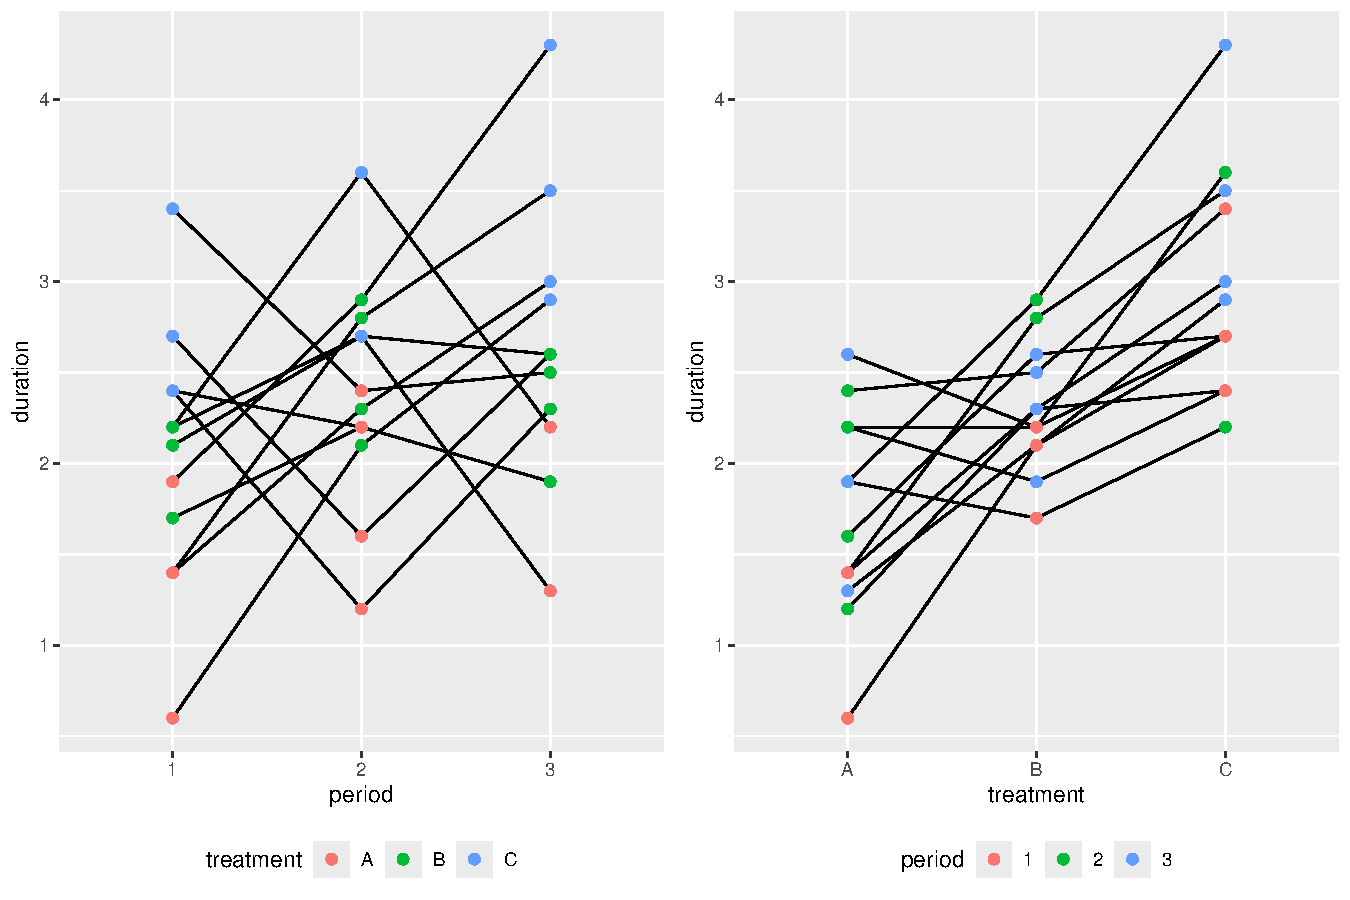
\includegraphics[trim={0 0 0 0},width=1\textwidth]{./figures/gg-spaghetti.pdf}
\end{center}

\clearpage
\section{Matching the t-test results}
\label{sec:org0555a47}

One can use a paired t-test to assess the treatment effect when there
is not missing values and no covariate to adjusted on (in particular
no period effect). It is easier to carry-out with the wide format of
the dataset:
\begin{lstlisting}[language=r,numbers=none]
bloodpressureW <- reshape(bloodpressureL, direction = "wide",
                          idvar = "id", timevar = "treatment",
                          v.names = c("duration","period"))
head(bloodpressureW)
\end{lstlisting}

\phantomsection
\label{}
\begin{verbatim}
   id sequence duration.A period.A duration.B period.B duration.C period.C
1   1      ABC        1.9        1        2.9        2        4.3        3
4   2      ABC        1.4        1        2.3        2        3.0        3
7   3      ABC        1.4        1        2.8        2        3.5        3
10  4      ABC        0.6        1        2.1        2        2.9        3
13  5      BCA        2.2        3        2.2        1        3.6        2
16  6      BCA        1.3        3        2.1        1        2.7        2
\end{verbatim}


For instance we can compare drug B and A using:
\begin{lstlisting}[language=r,numbers=none]
t.test(bloodpressureW$duration.B - bloodpressureW$duration.A)
\end{lstlisting}

\phantomsection
\label{}
\begin{verbatim}

	One Sample t-test

data:  bloodpressureW$duration.B - bloodpressureW$duration.A
t = 2.9, df = 11, p-value = 0.015
alternative hypothesis: true mean is not equal to 0
95 percent confidence interval:
 0.13805 1.01195
sample estimates:
mean of x 
    0.575
\end{verbatim}

To retrieve the same results with a linear mixed model, one can use
treatment as indexing the repetitions, i.e., model a treatment
specific variance and correlation:
\begin{lstlisting}[language=r,numbers=none]
eTreat.lmm2tt <- lmm(duration ~ treatment, repetition = ~treatment|id, data = bloodpressureL)
model.tables(eTreat.lmm2tt)
\end{lstlisting}

\phantomsection
\label{}
\begin{verbatim}
            estimate      se     df   lower  upper    p.value
(Intercept)   1.7250 0.16703 11.002 1.35739 2.0926 5.3415e-07
treatmentB    0.5750 0.19853 10.998 0.13804 1.0120 1.4542e-02
treatmentC    1.2583 0.22578 10.998 0.76137 1.7553 1.6701e-04
\end{verbatim}


\clearpage

\begin{description}
\item[{\Warning}] using period as the repetition variable, i.e., modeling a
period specific variance and correlation, would lead to different
estimates:
\end{description}
\begin{lstlisting}[language=r,numbers=none]
ePeriod.lmm2tt <- lmm(duration ~ treatment, repetition = ~period|id, data = bloodpressureL)
model.tables(ePeriod.lmm2tt)
\end{lstlisting}

\phantomsection
\label{}
\begin{verbatim}
            estimate      se      df   lower  upper    p.value
(Intercept)  1.68755 0.20349  4.7145 1.15478 2.2203 5.5048e-04
treatmentB   0.58766 0.19895 14.4584 0.16223 1.0131 1.0173e-02
treatmentC   1.16557 0.19654 11.9624 0.73718 1.5939 7.0104e-05
\end{verbatim}


As shown in appendix \ref{SM:lmm2average2}, this mixed model considers both
the variable treatment and period when deciding how much each
observation contributes to the estimation of a given parameter. On one
side, it makes sense that an observation taken at a period with large
variance should contribute less to parameter estimation compared to an
observation taken at a period with low variance. On the other side, it
can be suprising that treatment B outcomes can contribute to the
estimation of treatment A. This is however not the case in absence of
period effects since the weights sum to 0 for treatment B and C when
estimating the intercept.

\begin{description}
\item[{\Warning}] using a random intercept model instead would lead to the
same estimate but a different p-value:
\end{description}
\begin{lstlisting}[language=r,numbers=none]
eTreat.RI <- lmm(duration ~ treatment + (1|id), data = bloodpressureL)
model.tables(eTreat.RI)
\end{lstlisting}

\phantomsection
\label{}
\begin{verbatim}
            estimate      se     df   lower   upper    p.value
(Intercept)   1.7250 0.15192 29.483 1.41452 2.03548 2.7569e-12
treatmentB    0.5750 0.18673 22.000 0.18774 0.96226 5.4846e-03
treatmentC    1.2583 0.18673 22.000 0.87107 1.64560 8.9931e-07
\end{verbatim}


as it makes more restrictive assumptions (homoschedasticity, equal
correlation).

\clearpage
\section{Accounting for a period effect}
\label{sec:orgac4d037}

A natural extension of the t-test to adjust for a possible period
effect on the average outcome is to consider the corresponding mixed
model (i.e. treatment as repetition) and add period in the mean model:
\begin{lstlisting}[language=r,numbers=none]
eTreat.lmm <- lmm(duration ~ treatment + period, repetition = ~treatment|id,
                  data = bloodpressureL)
summary(eTreat.lmm)
\end{lstlisting}

\phantomsection
\label{}
\begin{verbatim}
		Linear Mixed Model 
 
Dataset: bloodpressureL 

  - 12 clusters 
  - 36 observations 
  - 3 observations per cluster 

Summary of the outcome and covariates: 

    $ duration : num  1.9 2.9 4.3 1.4 2.3 3 1.4 2.8 3.5 0.6 ...
    $ treatment: Factor w/ 3 levels "A","B","C": 1 2 3 1 2 3 1 2 3 1 ...
    $ period   : Factor w/ 3 levels "1","2","3": 1 2 3 1 2 3 1 2 3 1 ...
    reference level: treatment=A;period=1 

Estimation procedure 

  - Restricted Maximum Likelihood (REML) 
  - log-likelihood :-21.065
  - parameters: mean = 5, variance = 3, correlation = 3
  - convergence: TRUE (17 iterations) 
    largest |score| = 8.738e-05 for rho(A,B)
            |change|= 2.65176445995996e-06 for rho(A,B)
 
Residual variance-covariance: unstructured 

  - correlation structure: ~0 + treatment 
          A     B     C
    A 1.000 0.133 0.353
    B 0.133 1.000 0.759
    C 0.353 0.759 1.000

  - variance structure: ~treatment 
            standard.deviation ratio
    sigma.A              0.524 1.000
    sigma.B              0.330 0.629
    sigma.C              0.564 1.075

Fixed effects: duration ~ treatment + period 

               estimate    se   df  lower upper p.value    
   (Intercept)    1.549 0.166 13.9  1.193 1.905 < 1e-04 ***
   treatmentB     0.575 0.168  9.4  0.198 0.952 0.00707  **
   treatmentC     1.258 0.179  9.3  0.856 1.661 < 1e-04 ***
   period2          0.2 0.127    4 -0.151 0.551 0.18984    
   period3        0.328 0.121  4.9  0.014 0.641 0.04359   *
   ------------------------------------------------------- 
    :  0 '***' 0.001 '**' 0.01 '*' 0.05 '.' 0.1 ' ' 1.
  df: Satterthwaite approximation w.r.t. model-based se. 
  se: Modeled based on the observed information.
\end{verbatim}


Here because the design is balanced in term of period across
treatments, we obtain the same estimates for the difference in
treatment effect as if we do not adjust for period. However the
estimated mean outcome under each treatment (say treatment A) now
depends on all observations (and not only observations under treatment
A). See appendix \ref{SM:lmm2average3} for details.

\clearpage
\section{What if there is a baseline measurement?}
\label{sec:org53e67f9}

Consider now another study design where all patients have a baseline
measurement before receiving each treatment. As an illustrative
example we will consider the following illustrative dataset:
\begin{lstlisting}[language=r,numbers=none]
rho <- c(AB = 0.3, bb = 0.9, bA = 0.7, bB = 0.6)
SigmaBCO <- rbind(cbind(matrix(c(1,rho["bA"],rho["bA"],1),2,2),
                        matrix(c(rho["bb"],rho["bA"],rho["bB"],rho["AB"]),2,2)),
                  cbind(matrix(c(rho["bb"],rho["bB"],rho["bA"],rho["AB"]),2,2),
                        matrix(c(1,rho["bB"],rho["bB"],1),2,2)))
muBCO <- c(b1 = 0, A = 1, b2 = 0, B = 1.5)

library(mvtnorm)
set.seed(10)
n.obs <- 15
M1 <- data.frame(id = 1:n.obs, sequence = "AB",
                 rmvnorm(n.obs, mean = muBCO, sigma = SigmaBCO))
names(M1)[3:6] <- paste0("T",1:4)
M2 <- data.frame(id = n.obs+(1:n.obs), sequence = "BA",
                 rmvnorm(n.obs, mean = muBCO[c(1,4,3,2)],
                         sigma = SigmaBCO[c(1,4,3,2),c(1,4,3,2)]))
names(M2)[3:6] <- paste0("T",1:4)
dfL.BCO <- reshape(rbind(M1,M2), direction = "long",
                   idvar = "id", varying = names(M1)[-(1:2)], v.names = c("Y"), times = 1:4)
dfL.BCO$treatment <- "baseline"
dfL.BCO$treatment[dfL.BCO$time == 2 & dfL.BCO$sequence == "AB"] <- "A"
dfL.BCO$treatment[dfL.BCO$time == 4 & dfL.BCO$sequence == "AB"] <- "B"
dfL.BCO$treatment[dfL.BCO$time == 2 & dfL.BCO$sequence == "BA"] <- "B"
dfL.BCO$treatment[dfL.BCO$time == 4 & dfL.BCO$sequence == "BA"] <- "A"
dfL.BCO$treatment <- factor(dfL.BCO$treatment, levels = c("baseline","A","B"))
dfL.BCO$period <- as.character(1 + (dfL.BCO$time %in% 3:4))
dfL.BCO[dfL.BCO$id==1,]
\end{lstlisting}

\phantomsection
\label{}
\begin{verbatim}
    id sequence time        Y treatment period
1.1  1       AB    1 -0.84169  baseline      1
1.2  1       AB    2  0.36197         A      1
1.3  1       AB    3 -1.28127  baseline      2
1.4  1       AB    4  0.57369         B      2
\end{verbatim}



\begin{lstlisting}[language=r,numbers=none]
gg.BCO <- ggplot(dfL.BCO, aes(x=time, y = Y, group = id))
gg.BCO <- gg.BCO + geom_line()
gg.BCO <- gg.BCO + geom_point(aes(color = treatment, shape = treatment), size = 3)
gg.BCO <- gg.BCO + facet_wrap(~sequence, labeller = label_both)
gg.BCO
\end{lstlisting}

\begin{center}
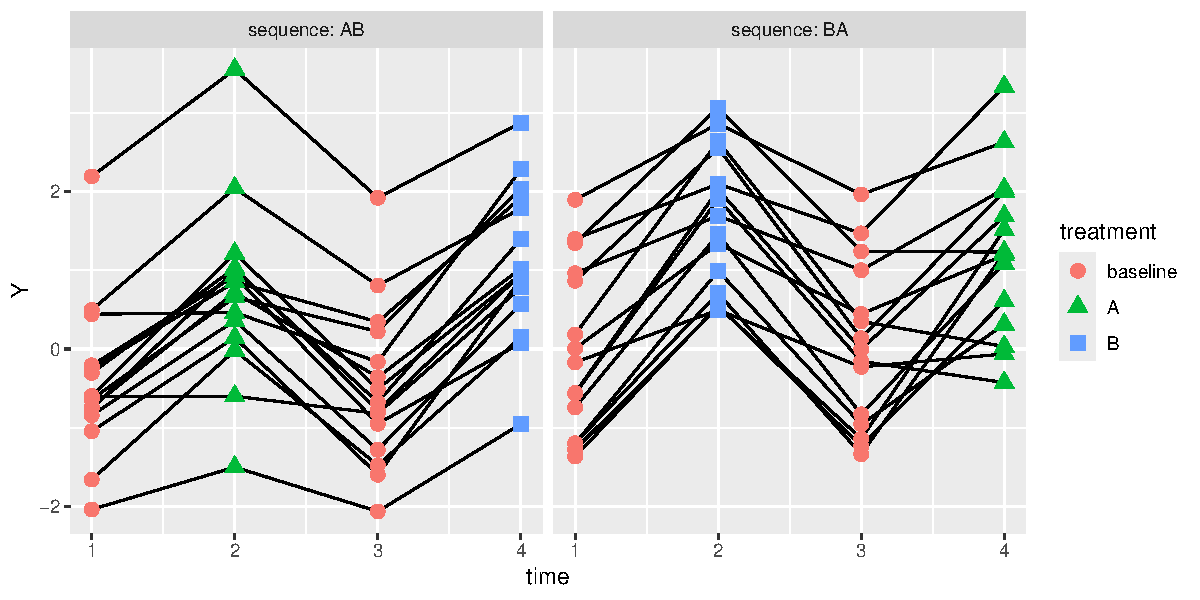
\includegraphics[trim={0 0 0 0},width=1\textwidth]{./figures/spa-BCO.pdf}
\end{center}
\subsection{First time period}
\label{sec:org69c7936}

If we restrict the dataset to the first period (time 1 and 2):
\begin{lstlisting}[language=r,numbers=none]
dfLred.BCO <- dfL.BCO[dfL.BCO$time %in% 1:2,]
\end{lstlisting}

\noindent we obtain a standard 2 arm randomized trial. A linear mixed
model with baseline constraint:
\begin{lstlisting}[language=r,numbers=none]
e0.lmm <- lmm(Y ~ treatment, repetition =~time|id, data = dfLred.BCO)
model.tables(e0.lmm)
\end{lstlisting}

\phantomsection
\label{}
\begin{verbatim}
            estimate      se     df    lower   upper    p.value
(Intercept) -0.23175 0.19023 29.005 -0.62081 0.15731 2.3294e-01
treatmentA   1.12010 0.15613 28.838  0.80070 1.43950 6.9791e-08
treatmentB   1.73010 0.15613 28.838  1.41070 2.04950 6.5641e-12
\end{verbatim}


estimates a treatment effect:
\begin{lstlisting}[language=r,numbers=none]
e0.lmm2ANCOVA <- anova(e0.lmm, effects = c("treatmentB-treatmentA=0"), multivariate=FALSE)
summary(e0.lmm2ANCOVA, digits = 5)
\end{lstlisting}

\phantomsection
\label{}
\begin{verbatim}
              Univariate Wald test 

                         estimate      se   df   lower   upper p.value   
 treatmentB-treatmentA=0     0.61 0.21653 27.8 0.16628 1.05372 0.00882 **
 ------------------------------------------------------------------------ 
  :  0 '***' 0.001 '**' 0.01 '*' 0.05 '.' 0.1 ' ' 1.
df: Satterthwaite approximation w.r.t. model-based se. 
se: Modeled based on the observed information.
\end{verbatim}


identical to an ANCOVA:
\begin{lstlisting}[language=r,numbers=none]
dfWred.BCO <- reshape(dfLred.BCO, direction = "wide",
                      timevar = "time", idvar = "id", v.names = c("Y","treatment"))
e.ANCOVA <- lm(Y.2 ~ Y.1 + treatment.2, data = dfWred.BCO)
summary(e.ANCOVA)$coef
\end{lstlisting}

\phantomsection
\label{}
\begin{verbatim}
             Estimate Std. Error t value   Pr(>|t|)
(Intercept)   1.07449    0.15983  6.7226 3.2294e-07
Y.1           0.80321    0.10762  7.4631 4.9918e-08
treatment.2B  0.61000    0.22050  2.7664 1.0103e-02
\end{verbatim}


\Warning When fitting the mixed model, the variance was on purpose
modeled to be time dependent instead of treatment dependent to match
the ANCOVA. In many applications, however, a treatment dependent
variance and correlation is preferable:
\begin{lstlisting}[language=r,numbers=none]
e0T.lmm <- lmm(Y ~ treatment, repetition =~treatment|id, data = dfLred.BCO)
e0T.lmm2ANCOVA <- anova(e0T.lmm, effects = c("treatmentB-treatmentA=0"), multivariate=FALSE)
summary(e0T.lmm2ANCOVA, digits = 5)
\end{lstlisting}

\phantomsection
\label{}
\begin{verbatim}
              Univariate Wald test 

                         estimate      se   df   lower   upper p.value   
 treatmentB-treatmentA=0  0.60238 0.21631 27.7 0.15909 1.04567 0.00954 **
 ------------------------------------------------------------------------ 
  :  0 '***' 0.001 '**' 0.01 '*' 0.05 '.' 0.1 ' ' 1.
df: Satterthwaite approximation w.r.t. model-based se. 
se: Modeled based on the observed information.
\end{verbatim}


\textbf{Covariates}: to retrieve the same point estimate between the ANCOVA
and the mixed model, covariates should be included in the mixed model
with a time interaction.
\subsection{Multiple time periods}
\label{sec:orgcf3dcd6}

When considering multiple time periods one can use a similar mixed
model as before, possibly adjusting for a period effect:
\begin{lstlisting}[language=r,numbers=none]
eBCO.lmm <- lmm(Y ~ 0 + period + treatment, repetition =~time|id, data = dfL.BCO)
model.tables(eBCO.lmm)
\end{lstlisting}

\phantomsection
\label{}
\begin{verbatim}
           estimate      se     df    lower   upper    p.value
period1    -0.23365 0.18998 28.939 -0.62225 0.15494 2.2866e-01
period2    -0.22767 0.18847 28.829 -0.61324 0.15790 2.3687e-01
treatmentA  1.19661 0.12208 52.831  0.95173 1.44148 1.7431e-13
treatmentB  1.62931 0.12235 52.956  1.38389 1.87472 0.0000e+00
\end{verbatim}


The corresponding treatment effect over both period is then:
\begin{lstlisting}[language=r,numbers=none]
eBCO.lmm2ANCOVA <- anova(eBCO.lmm, effects = c("treatmentB-treatmentA=0"), multivariate=FALSE)
summary(eBCO.lmm2ANCOVA, digits = 5)
\end{lstlisting}

\phantomsection
\label{}
\begin{verbatim}
              Univariate Wald test 

                         estimate      se   df   lower   upper p.value  
 treatmentB-treatmentA=0   0.4327 0.17556 26.5 0.07213 0.79327  0.0205 *
 ----------------------------------------------------------------------- 
  :  0 '***' 0.001 '**' 0.01 '*' 0.05 '.' 0.1 ' ' 1.
df: Satterthwaite approximation w.r.t. model-based se. 
se: Modeled based on the observed information.
\end{verbatim}


This is close, but not identical to, averaging the ANCOVA treatment
effect estimates over periods:
\begin{lstlisting}[language=r,numbers=none]
dfWred2.BCO <- reshape(dfL.BCO[dfL.BCO$time %in% 3:4,], direction = "wide",
                      timevar = "time", idvar = "id", v.names = c("Y","treatment"))
e.ANCOVA2 <- lm(Y.4 ~ Y.3 + treatment.4, data = dfWred2.BCO)
mean(c(summary(e.ANCOVA)$coef[3,"Estimate"],summary(e.ANCOVA2)$coef[3,"Estimate"]))
\end{lstlisting}

\phantomsection
\label{}
\begin{verbatim}
[1] 0.43672
\end{verbatim}


\Warning In many applications, however, a treatment dependent variance
and correlation is preferable:
\begin{lstlisting}[language=r,numbers=none]
eBCOT.lmm <- lmm(Y ~ 0 + period + treatment, repetition =~time|id,
                 structure = CS(list(~treatment,~treatment)), data = dfL.BCO)
model.tables(eBCOT.lmm, effects = "all")
\end{lstlisting}

\phantomsection
\label{}
\begin{verbatim}
                estimate       se     df    lower   upper    p.value
period1         -0.22434 0.190420 30.812 -0.61280 0.16412 2.4776e-01
period2         -0.22920 0.190420 30.812 -0.61767 0.15926 2.3788e-01
treatmentA       1.20288 0.138802 28.981  0.91899 1.48677 1.5370e-09
treatmentB       1.61662 0.103330 28.960  1.40527 1.82797 1.1102e-15
sigma            1.04573 0.132524 21.199  0.80358 1.36086         NA
k.A              1.05138 0.128001 35.720  0.82129 1.34593 6.8315e-01
k.B              0.91362 0.091255 33.724  0.74573 1.11930 3.7216e-01
rho(baseline)    0.92897 0.025392 43.269  0.85573 0.96572 2.4213e-11
rho(baseline,A)  0.73301 0.082718 23.079  0.51201 0.86300 2.6062e-05
rho(baseline,B)  0.82435 0.056386 26.233  0.66887 0.91073 4.4893e-07
rho(A,B)         0.58845 0.121439 19.844  0.27992 0.78680 1.6645e-03
\end{verbatim}

leading to the following treatment effect estimate:
\begin{lstlisting}[language=r,numbers=none]
eBCOT.lmm2ANCOVA <- anova(eBCOT.lmm, effects = c("treatmentB-treatmentA=0"),
                          multivariate=FALSE)
summary(eBCOT.lmm2ANCOVA, digits = 5)
\end{lstlisting}

\phantomsection
\label{}
\begin{verbatim}
             Univariate Wald test 

                         estimate      se df   lower  upper p.value  
 treatmentB-treatmentA=0  0.41374 0.17179 29 0.06237 0.7651  0.0226 *
 -------------------------------------------------------------------- 
  :  0 '***' 0.001 '**' 0.01 '*' 0.05 '.' 0.1 ' ' 1.
df: Satterthwaite approximation w.r.t. model-based se. 
se: Modeled based on the observed information.
\end{verbatim}



\noindent If, instead of the ANCOVA, the change from baseline between
treatments is of interest:
\begin{lstlisting}[language=r,numbers=none]
dfW.BCO <- reshape(dfL.BCO, direction = "wide",
                   timevar = "time", idvar = "id", v.names = c("Y","period","treatment"))
dfW.BCO$dY <- (dfW.BCO$Y.4-dfW.BCO$Y.3)-(dfW.BCO$Y.2-dfW.BCO$Y.1)
t.test(c(dfW.BCO$dY[dfW.BCO$sequence == "AB"],-dfW.BCO$dY[dfW.BCO$sequence == "BA"]))
\end{lstlisting}

\phantomsection
\label{}
\begin{verbatim}

	One Sample t-test

data:  c(dfW.BCO$dY[dfW.BCO$sequence == "AB"], -dfW.BCO$dY[dfW.BCO$sequence == "BA"])
t = 2.64, df = 29, p-value = 0.013
alternative hypothesis: true mean is not equal to 0
95 percent confidence interval:
 0.10826 0.85027
sample estimates:
mean of x 
  0.47927
\end{verbatim}

one can retrieve this results by introducing 2 new design variables:
\begin{lstlisting}[language=r,numbers=none]
dfL.BCO$treated <- (dfL.BCO$treatment!="baseline")
dfL.BCO$periodB <- with(dfL.BCO, (period==1 & sequence=="BA") | (period==2 & sequence=="AB"))
e.lmm2tt <- lmm(Y ~ sequence:treated+(treated*periodB),
                repetition = ~time|id, data = dfL.BCO)
model.tables(e.lmm2tt)
\end{lstlisting}

\phantomsection
\label{}
\begin{verbatim}
                        estimate       se     df    lower    upper    p.value
(Intercept)             -0.43409 0.264062 28.838 -0.97429 0.106105 1.1105e-01
treatedTRUE              1.14741 0.140692 35.009  0.86179 1.433027 1.3152e-09
periodBTRUE             -0.06553 0.071101 28.992 -0.21095 0.079889 3.6432e-01
sequenceBA:treatedFALSE  0.47492 0.370826 28.037 -0.28463 1.234483 2.1079e-01
sequenceBA:treatedTRUE   0.52510 0.325697 28.013 -0.14205 1.192241 1.1812e-01
treatedTRUE:periodBTRUE  0.47927 0.181401 28.988  0.10825 0.850279 1.3146e-02
\end{verbatim}


where the coefficient of interest in the last line, among the
treatment periods (A or B) whether there is a difference between being
under treatment B or treatment A.

\clearpage

\appendix
\titleformat{\section}
{\normalfont\Large\bfseries}{Appendix~\thesection}{1em}{}

\renewcommand{\thefigure}{\Alph{figure}}
\renewcommand{\thetable}{\Alph{table}}
\renewcommand{\theequation}{\Alph{equation}}

\setcounter{figure}{0}    
\setcounter{table}{0}    
\setcounter{equation}{0}    
\section{Mixed model estimator as a weighted average}
\label{SM:lmm2average}
\subsection{Treatment as repetition variable}
\label{SM:lmm2average1}
Consider the linear mixed model matching the t-test results when
estimating the treatment effect:
\begin{lstlisting}[language=r,numbers=none]
eTreat.lmm2tt <- lmm(duration ~ treatment, repetition = ~treatment|id, data = bloodpressureL)
coef(eTreat.lmm2tt)
\end{lstlisting}

\phantomsection
\label{}
\begin{verbatim}
(Intercept)  treatmentB  treatmentC 
     1.7250      0.5750      1.2583
\end{verbatim}


\noindent The estimates correspond to a Generalized Least Squared (GLS)
estimator defined by:

\smallskip

\begin{minipage}[t]{0.55\linewidth}
\begin{itemize}
\item a block diagonal covariance matrix with element
\end{itemize}
\begin{lstlisting}[language=r,numbers=none]
Omega1 <- sigma(eTreat.lmm2tt,
               cluster = "all", simplify = TRUE)
Omega1[1:3,1:3]
\end{lstlisting}

\phantomsection
\label{}
\begin{verbatim}
           [,1]       [,2]     [,3]
[1,]  0.3347727 -0.0072727 0.047727
[2,] -0.0072727  0.1236364 0.162727
[3,]  0.0477273  0.1627273 0.372424
\end{verbatim}

\end{minipage}
\begin{minipage}[t]{0.02\linewidth}
\hphantom{x}
\end{minipage}
\begin{minipage}[t]{0.4\linewidth}
\begin{itemize}
\item a design matrix with element:
\end{itemize}
\begin{lstlisting}[language=r,numbers=none]
X1 <- model.matrix(eTreat.lmm2tt)
head(X1,3)
\end{lstlisting}

\phantomsection
\label{}
\begin{verbatim}
  (Intercept) treatmentB treatmentC
1           1          0          0
2           1          1          0
3           1          0          1
\end{verbatim}

\end{minipage}

\noindent The corresponding projector weight each observation:
\begin{itemize}
\item proportionally to the sample size for treatments related to the regression parameter
\item 0 otherwise:
\end{itemize}

\begin{lstlisting}[language=r,numbers=none]
P1 <- solve(t(X1) %*% solve(Omega1) %*% X1) %*% t(X1) %*% solve(Omega1)
vecP1 <- apply(round(P1,4), MARGIN = 1, FUN = table, y = bloodpressureL$treatment)
vecP1
\end{lstlisting}

\begin{minipage}{0.3\linewidth}
\phantomsection
\label{}
\begin{verbatim}
$`(Intercept)`
        A  B  C
0       0 12 12
0.0833 12  0  0
total   1  0  0
\end{verbatim}


\end{minipage}
\begin{minipage}{0.3\linewidth}
\phantomsection
\label{}
\begin{verbatim}
$treatmentB
         A  B  C
-0.0833 12  0  0
0        0  0 12
0.0833   0 12  0
total   -1  1  0
\end{verbatim}

\end{minipage}
\begin{minipage}{0.3\linewidth}
\phantomsection
\label{}
\begin{verbatim}
$treatmentC
         A  B  C
-0.0833 12  0  0
0        0 12  0
0.0833   0  0 12
total   -1  0  1
\end{verbatim}

\end{minipage}



\noindent We can verify that we retrieve the mixed model estimates:
\begin{lstlisting}[language=r,numbers=none]
(P1 %*% bloodpressureL$duration)[,1]
\end{lstlisting}

\phantomsection
\label{}
\begin{verbatim}
(Intercept)  treatmentB  treatmentC 
     1.7250      0.5750      1.2583
\end{verbatim}


\clearpage
\subsection{Period as repetition variable}
\label{SM:lmm2average2}
Consider the same linear mixed model but with period as repetition variable:
\begin{lstlisting}[language=r,numbers=none]
ePeriod.lmm2tt <- lmm(duration ~ treatment, repetition = ~period|id, data = bloodpressureL)
coef(ePeriod.lmm2tt)
\end{lstlisting}

\phantomsection
\label{}
\begin{verbatim}
(Intercept)  treatmentB  treatmentC 
    1.68755     0.58766     1.16557
\end{verbatim}


\noindent The estimates correspond to a Generalized Least Squared (GLS)
estimator defined by:

\smallskip


\begin{minipage}[t]{0.55\linewidth}
\begin{itemize}
\item a block diagonal covariance matrix with elements
\end{itemize}
\begin{lstlisting}[language=r,numbers=none]
Omega2 <- sigma(ePeriod.lmm2tt,
               cluster = "all", simplify = TRUE)
Omega2[1:3,1:3]
\end{lstlisting}

\phantomsection
\label{}
\begin{verbatim}
         [,1]     [,2]    [,3]
[1,] 0.229440 0.082455 0.01444
[2,] 0.082455 0.249826 0.11704
[3,] 0.014440 0.117040 0.36480
\end{verbatim}


\end{minipage}
\begin{minipage}[t]{0.02\linewidth}
\hphantom{x}
\end{minipage}
\begin{minipage}[t]{0.4\linewidth}
\begin{itemize}
\item a design matrix with element:
\end{itemize}
\begin{lstlisting}[language=r,numbers=none]
X2 <- model.matrix(eTreat.lmm2tt)
X2[1:3,1:3]
\end{lstlisting}

\phantomsection
\label{}
\begin{verbatim}
  (Intercept) treatmentB treatmentC
1           1          0          0
2           1          1          0
3           1          0          1
\end{verbatim}

\end{minipage}

\noindent The weigthing of the observations is less intuitive as all
treatments contribute, to various extends, to each regression parameter.

\begin{lstlisting}[language=r,numbers=none]
P2 <- solve(t(X2) %*% solve(Omega2) %*% X2) %*% t(X2) %*% solve(Omega2)
vecP2 <- apply(round(P2,4), MARGIN = 1, FUN = table, y = bloodpressureL$treatment,
               simplify = FALSE)
\end{lstlisting}

\begin{minipage}{0.3\linewidth}
\phantomsection
\label{}
\begin{verbatim}
$`(Intercept)`
        A B C
-0.0156 0 4 0
-0.0129 0 0 4
-0.0123 0 4 0
-0.0053 0 0 4
0.0182  0 0 4
0.0279  0 4 0
0.0611  4 0 0
0.0922  4 0 0
0.0967  4 0 0
total   1 0 0
\end{verbatim}

\end{minipage}
\begin{minipage}{0.3\linewidth}
\phantomsection
\label{}
\begin{verbatim}
$treatmentB
         A B C
-0.1052  4 0 0
-0.102   4 0 0
-0.0429  4 0 0
-0.0306  0 0 4
-0.0026  0 0 4
0.0332   0 0 4
0.0688   0 4 0
0.0734   0 4 0
0.1078   0 4 0
total   -1 1 0
\end{verbatim}
\end{minipage}
\begin{minipage}{0.3\linewidth}
\phantomsection
\label{}
\begin{verbatim}
$treatmentC
         A B C
-0.1078  4 0 0
-0.0734  4 0 0
-0.0688  4 0 0
-0.0332  0 4 0
0.0026   0 4 0
0.0306   0 4 0
0.0429   0 0 4
0.102    0 0 4
0.1052   0 0 4
total   -1 0 1
\end{verbatim}
\end{minipage}

\noindent We can verify that we retrieve the mixed model estimates:
\begin{lstlisting}[language=r,numbers=none]
(P2 %*% bloodpressureL$duration)[,1]
\end{lstlisting}

\phantomsection
\label{}
\begin{verbatim}
(Intercept)  treatmentB  treatmentC 
    1.68755     0.58766     1.16557
\end{verbatim}
\subsection{Treatment as repetition variable, adjusted for period}
\label{SM:lmm2average3}
We now consider the linear mixed model similar to the t-test but
adjusting for period:
\begin{lstlisting}[language=r,numbers=none]
eTreat.lmm <- lmm(duration ~ treatment + period, repetition = ~treatment|id,
                  data = bloodpressureL)
coef(eTreat.lmm)
\end{lstlisting}

\phantomsection
\label{}
\begin{verbatim}
(Intercept)  treatmentB  treatmentC     period2     period3 
    1.54915     0.57500     1.25833     0.19991     0.32764
\end{verbatim}


As before we extract the residual-variance covariance matrix and the
design matrix:
\begin{lstlisting}[language=r,numbers=none]
Omega3 <- sigma(eTreat.lmm,
               cluster = "all", simplify = TRUE)
X3 <- model.matrix(eTreat.lmm)
\end{lstlisting}

\noindent to understand how the GLS estimator weight each observation:

\begin{lstlisting}[language=r,numbers=none]
P3 <- solve(t(X3) %*% solve(Omega3) %*% X3) %*% t(X3) %*% solve(Omega3)
vecP3 <- apply(round(P3,4), MARGIN = 1, FUN = table, y = bloodpressureL$treatment)
vecP3
\end{lstlisting}

\begin{minipage}{0.3\linewidth}
\phantomsection
\label{}
\begin{verbatim}
$`(Intercept)`
        A B C
-0.0828 0 4 0
-0.0497 0 0 4
-0.0134 0 4 0
-0.0048 0 0 4
0.0546  0 0 4
0.0631  4 0 0
0.0876  4 0 0
0.0962  0 4 0
0.0992  4 0 0
total   1 0 0
\end{verbatim}

\end{minipage}
\begin{minipage}{0.3\linewidth}
\phantomsection
\label{}
\begin{verbatim}
$treatmentB
         A  B  C
-0.0833 12  0  0
0        0  0 12
0.0833   0 12  0
total   -1  1  0
\end{verbatim}

\end{minipage}
\begin{minipage}{0.3\linewidth}
\phantomsection
\label{}
\begin{verbatim}
$treatmentC
         A  B  C
-0.0833 12  0  0
0        0 12  0
0.0833   0  0 12
total   -1  0  1
\end{verbatim}

\end{minipage}



\noindent We can verify that we retrive the mixed model estimates:
\begin{lstlisting}[language=r,numbers=none]
(P3 %*% bloodpressureL$duration)[,1]
\end{lstlisting}

\phantomsection
\label{}
\begin{verbatim}
(Intercept)  treatmentB  treatmentC     period2     period3 
    1.54915     0.57500     1.25833     0.19991     0.32764
\end{verbatim}


\clearpage
\subsection{Period as repetition variable, adjusted for period}
\label{SM:lmm2average4}
We now consider the linear mixed model similar to the t-test but
adjusting for period:
\begin{lstlisting}[language=r,numbers=none]
ePeriod.lmm <- lmm(duration ~ treatment + period, repetition = ~period|id,
                  data = bloodpressureL)
coef(ePeriod.lmm)
\end{lstlisting}

\phantomsection
\label{}
\begin{verbatim}
(Intercept)  treatmentB  treatmentC     period2     period3 
    1.31867     0.74657     1.39742     0.35833     0.55000
\end{verbatim}


As before we extract the residual-variance covariance matrix and the
design matrix:
\begin{lstlisting}[language=r,numbers=none]
Omega4 <- sigma(ePeriod.lmm,
               cluster = "all", simplify = TRUE)
X4 <- model.matrix(ePeriod.lmm)
\end{lstlisting}

\noindent to understand how the GLS estimator weight each observation:

\begin{lstlisting}[language=r,numbers=none]
P4 <- solve(t(X4) %*% solve(Omega4) %*% X4) %*% t(X4) %*% solve(Omega4)
vecP4 <- apply(round(P4,4), MARGIN = 1, FUN = table, y = bloodpressureL$treatment)
vecP4
\end{lstlisting}

\begin{minipage}{0.3\linewidth}
\phantomsection
\label{}
\begin{verbatim}
$`(Intercept)`
        A B C
-0.0442 0 4 0
-0.0385 0 0 4
0.0032  0 4 0
0.0035  0 0 4
0.035   0 0 4
0.0353  4 0 0
0.0407  4 0 0
0.041   0 4 0
0.1739  4 0 0
total   1 0 0
\end{verbatim}

\end{minipage}
\begin{minipage}{0.3\linewidth}
\phantomsection
\label{}
\begin{verbatim}
$treatmentB
         A B C
-0.1389  4 0 0
-0.0738  4 0 0
-0.0477  0 0 4
-0.0373  4 0 0
0.006    0 0 4
0.0321   0 4 0
0.0417   0 0 4
0.0849   0 4 0
0.1329   0 4 0
total   -1 1 0
\end{verbatim}
\end{minipage}
\begin{minipage}{0.3\linewidth}
\phantomsection
\label{}
\begin{verbatim}
$treatmentC
         A B C
-0.1329  4 0 0
-0.0849  4 0 0
-0.0417  0 4 0
-0.0321  4 0 0
-0.006   0 4 0
0.0373   0 0 4
0.0477   0 4 0
0.0738   0 0 4
0.1389   0 0 4
total   -1 0 1
\end{verbatim}
\end{minipage}



\noindent We can verify that we retrieve the mixed model estimates:
\begin{lstlisting}[language=r,numbers=none]
(P4 %*% bloodpressureL$duration)[,1]
\end{lstlisting}

\phantomsection
\label{}
\begin{verbatim}
(Intercept)  treatmentB  treatmentC     period2     period3 
    1.31867     0.74657     1.39742     0.35833     0.55000
\end{verbatim}
\end{document}
